\documentclass[conference]{IEEEtran}
\usepackage{cite,amsmath,graphicx,booktabs,xcolor,url,hyperref}
\newcommand{\TODO}[1]{\textcolor{red}{[TODO: #1]}}
% macros auto-filled by src/make_tables.py (placeholders until runs finish)
\newcommand{\resBaseITW}{XX.XX}\newcommand{\resBaseLA}{XX.XX}\newcommand{\resOursITW}{XX.XX}
\newcommand{\resOursLA}{XX.XX}\newcommand{\resOursTDCF}{X.XXX}\newcommand{\resLfccITW}{XX.XX}\newcommand{\resRel}{XX}
\IfFileExists{results_macros.tex}{\renewcommand{\resBaseITW}{19.67}
\renewcommand{\resBaseLA}{5.56}
\renewcommand{\resOursITW}{14.00}
\renewcommand{\resOursLA}{1.67}
\renewcommand{\resOursTDCF}{0.037}
\renewcommand{\resLfccITW}{62.33}
\renewcommand{\resRel}{29}
}{}
\IfFileExists{results_tables.tex}{}{\newcommand{\missingtab}{}}

\begin{document}
\title{Generalizable Audio Deepfake Detection: Cross-Dataset Spoofed-Speech Detection using Self-Supervised Speech Representations}
\author{\IEEEauthorblockN{Thakshaya, S Mahadhevan, Satya P, V Shalini, Vishal M}
\IEEEauthorblockA{Department of Information Technology, PSG College of Technology, Coimbatore, India\\
Contact: \texttt{23i348@psgtech.ac.in}}}
\date{}
\maketitle

\begin{abstract}
Audio deepfake detectors trained on ASVspoof~2019 Logical Access (LA) reach low in-domain equal error rates (EER) but degrade sharply on real-world recordings. We train only on LA and test on the In-the-Wild (ITW) corpus, studying three components on a frozen WavLM front end: (i) learned softmax fusion of all transformer layers with attentive-statistics pooling (LAF), (ii) codec, channel and noise augmentation, and (iii) a gradient-reversal head that encourages invariance to the augmentation domain (CoLA). Using frozen WavLM-base-plus features and class-balanced evaluation subsets, LAF reduces EER from 5.6\% to 2.2\% on LA eval and from 19.7\% to 15.7\% on ITW relative to a last-layer baseline; augmentation further lowers ITW EER to 13.9\%. The adversarial head gave no measurable additional gain (14.0\%), and a fixed uniform layer average performed comparably to learned weights (14.8\%). A cross-dataset gap of about 12 EER points remains. We report ablations, per-attack analysis and learned layer weights.
\end{abstract}
\begin{IEEEkeywords}audio deepfake detection, anti-spoofing, self-supervised learning, WavLM, domain generalization, ASVspoof\end{IEEEkeywords}

\section{Introduction}
Neural text-to-speech and voice conversion now produce speech that listeners and speaker-verification systems often accept as genuine, motivating countermeasures (CMs) for spoofed speech~\cite{yi2023survey}. Benchmarks such as ASVspoof~2019~\cite{wang2020asvspoof2019} drove rapid progress, and self-supervised learning (SSL) front ends have recently pushed in-domain EER below 1\%~\cite{tak2022wav2vec,wang2022investigating}. However, Müller \emph{et al.}~\cite{muller2022does} showed that models trained on ASVspoof data can perform far worse on audio collected from the internet, where recording conditions, codecs, languages and generators differ from the lab data. This \emph{generalization gap}, rather than in-domain accuracy, is the open problem.

We ask: \emph{how much of the cross-dataset gap can be closed with an SSL front end plus codec/noise-aware training, without using any In-the-Wild data for training or model selection?} Our contributions:
\begin{itemize}
\item A lightweight detector combining learned all-layer fusion (LAF) of a frozen SSL model, attentive-statistics pooling, codec/noise augmentation and an optional codec/noise-adversarial head (CoLA).
\item A controlled ablation isolating each component, including a negative result for the adversarial head.
\item A strict LA$\rightarrow$ITW protocol with multi-seed statistics, bootstrap confidence intervals, per-attack error analysis and layer-weight interpretation.
\end{itemize}

\section{Related Work}
\textbf{SSL front ends.} wav2vec~2.0~\cite{baevski2020wav2vec}, XLS-R~\cite{babu2022xlsr} and WavLM~\cite{chen2022wavlm} give strong features for spoof detection. Tak \emph{et al.} fine-tuned wav2vec~2.0 XLS-R with RawBoost augmentation and an AASIST back end~\cite{tak2022wav2vec,tak2022rawboost,jung2022aasist}; Wang and Yamagishi systematically compared SSL front ends~\cite{wang2022investigating}, and Mart{\'\i}n-Do{\~n}as and {\'A}lvarez used wav2vec2 for the 2022 ADD challenge~\cite{martin2022vicomtech}. Later work showed that which layers are used matters: the SLS classifier fuses layerwise XLS-R information~\cite{zhang2024sls}; Pascu \emph{et al.} study generalisation and calibration of SSL-based detectors~\cite{pascu2024towards}; and WavLM ensembles performed well in ASVspoof~5~\cite{combei2024wavlm}. Whisper features have also been used~\cite{kawa2023whisper}.\\
\textbf{Generalization and data.} ASVspoof~2021 added channel/codec and deepfake conditions~\cite{liu2023asvspoof2021}; ASVspoof~5 scales to crowdsourced data and adversarial attacks~\cite{wang2024asvspoof5}. Wang and Yamagishi created spoofed training data with neural vocoders~\cite{wang2023vocoded,wang2024largescale}, Codecfake targets neural-codec-based speech~\cite{xu2024codecfake}, and Ba \emph{et al.} study cross-language transfer~\cite{ba2023transferring}. Kawa \emph{et al.} examine adversarial robustness~\cite{kawa2023defense}. Earlier raw-waveform and graph-attention CMs include RawNet2 and AASIST~\cite{tak2021rawnet2,jung2022aasist}.\\
\textbf{Gap.} Prior work either improves features/back ends, or adds data/augmentation, but does not explicitly \emph{regularize the embedding to be invariant} to the nuisance domains that augmentation introduces. We combine layerwise SSL fusion with domain-adversarial training~\cite{ganin2015dann} using augmentation type as the nuisance label, and quantify the benefit under a strict train-on-LA, test-on-ITW protocol with $\geq$3 matched baselines and ablations.

\section{Datasets and Pre-processing}
\textbf{ASVspoof~2019 LA}~\cite{wang2020asvspoof2019}: 16\,kHz FLAC speech with six training attacks (A01--A06) and thirteen evaluation attacks (A07--A19, of which A16/A19 repeat A04/A06). Partitions are speaker-disjoint; our code asserts this at start-up. We train on \texttt{train}, select checkpoints on \texttt{dev}, and report on \texttt{eval}.\\
\textbf{In-the-Wild (ITW)}~\cite{muller2022does}: audio of public figures (bona fide and deepfakes) collected from the internet; used \emph{only} for testing. It has no ASV scores, so only EER is reported there.\\
\textbf{Pre-processing.} Audio is mono, 16\,kHz, fixed to 64\,600 samples ($\approx$4\,s; random crop in training, first segment at test, tiling for short clips) and per-utterance mean/variance normalized. Fig.~\ref{fig:eda} summarizes durations.\\
\textbf{Augmentation.} Each training clip is, with probability 0.2, left clean (domain 0); otherwise (domain 1) it receives RawBoost-style band-limited FIR filtering, soft non-linear distortion and/or coloured noise at 5--30\,dB SNR, or (domain 2) codec/channel simulation: $\mu$-law 8\,kHz telephony, MP3 (16--64\,kbps) and Opus (8--24\,kbps) via FFmpeg. Augmentation is applied only to training data.

\begin{figure}[t]\centering\IfFileExists{figs/fig_eda.pdf}{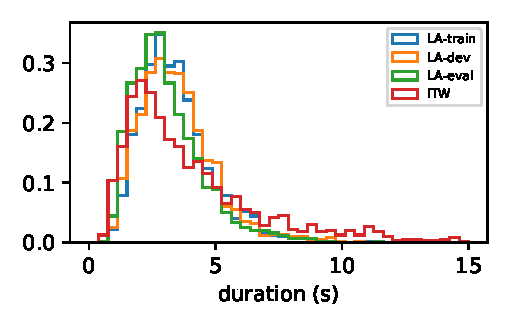
\includegraphics[width=.8\columnwidth]{figs/fig_eda.pdf}}{\fbox{EDA figure}}\caption{Duration distributions of the LA partitions and In-the-Wild.}\label{fig:eda}\end{figure}

\section{Proposed Method: CoLA-SSL}
Fig.~\ref{fig:arch} shows the model. A frozen SSL encoder yields hidden states $\{\mathbf h^{(l)}\}_{l=0}^{L}$. Layer fusion (LAF) forms $\mathbf z_t=\sum_l \alpha_l \mathbf h_t^{(l)}$ with $\boldsymbol\alpha=\mathrm{softmax}(\mathbf a)$ learned jointly; $\mathbf z$ is projected to 256-D and aggregated by attentive statistics pooling (attention-weighted mean and standard deviation) to an embedding $\mathbf f$. A classifier predicts bona fide vs.\ spoof. A second head predicts the augmentation domain $d\in\{0,1,2\}$ from $\mathbf f$ through a gradient-reversal layer (GRL)~\cite{ganin2015dann}. The loss is
\begin{equation}\mathcal L=\mathrm{CE}_w(y,\hat y)+\lambda_{\mathrm{adv}}\,\mathrm{CE}(d,\hat d),\end{equation}
with class weights $[0.1,0.9]$ (spoof, bona fide), $\lambda_{\mathrm{adv}}=0.3$ and the GRL coefficient ramped from 0 to 1 with the DANN schedule. The GRL pushes $\mathbf f$ to carry information that discriminates bona fide from spoofed speech but not the codec/noise condition. Only the fusion/pooling/classifier layers ($\sim$1\,M parameters) are trained, making training cheap.

\begin{figure*}[t]\centering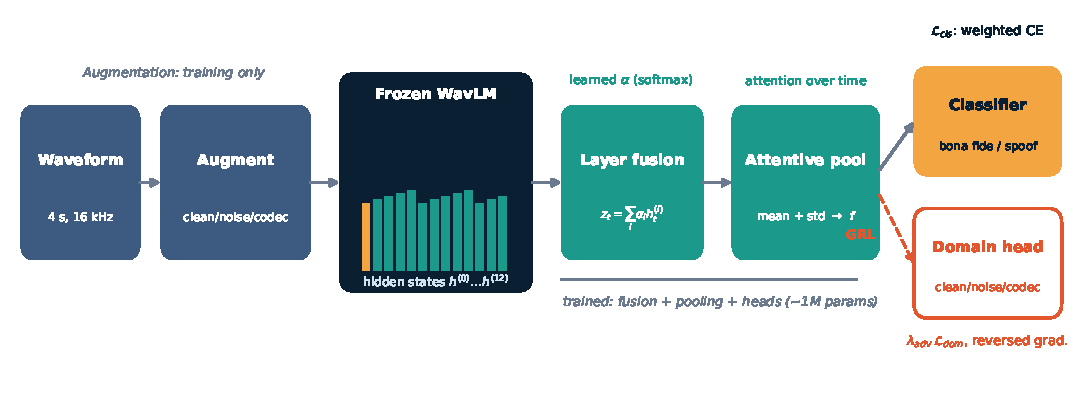
\includegraphics[width=0.92\textwidth]{figs/fig_arch.pdf}\caption{CoLA-SSL architecture. A frozen WavLM encoder yields 13 hidden-state layers, which are fused with learned softmax weights $\alpha_l$ and pooled by attentive statistics into an embedding $f$. A classifier predicts bona fide vs.\ spoof; during training an auxiliary domain head, connected through a gradient-reversal layer (GRL), predicts the augmentation type (clean, noise, codec). Only the fusion, pooling and head parameters are trained.}\label{fig:arch}\end{figure*}

\section{Experimental Setup}
\textbf{Baselines (same data, schedule and selection):} WavLM-base-plus with last-layer mean pooling and a linear head; an LFCC-LCNN non-SSL reference (single run, 1000 training clips, 15 epochs; a weak reference rather than a tuned system). \textbf{Ablations:} + LAF, + augmentation, + adversarial head. \textbf{Training (CPU budget):} frozen WavLM-base-plus features are extracted once from random class-balanced subsets of LA train/dev/eval and In-the-Wild (1000 training clips plus one augmented copy of each, 300 dev, 600 LA-eval and 600 ITW clips) and the heads are trained on this cache. AdamW, one-cycle LR (peak $10^{-3}$), batch 64, 30 epochs, best epoch by LA dev EER, 3 seeds; training uses 1000 class-balanced clips plus one augmented copy of each. \textbf{Metrics:} EER and min t-DCF~\cite{kinnunen2018tdcf} (ASVspoof~2019 cost parameters, ASV at its EER operating point; LA only), mean$\pm$std over seeds and 95\% bootstrap CIs. Published numbers for AASIST/SSL-AASIST~\cite{jung2022aasist,tak2022wav2vec} use different training protocols and are therefore not placed in the table.

\section{Results}
\IfFileExists{results_tables.tex}{\begin{table}[t]\centering\caption{Train on ASVspoof 2019 LA; EER (\%) on LA eval (in-domain) and In-the-Wild (cross-dataset). Mean$\pm$std over seeds. Gap = ITW EER $-$ LA EER (points). min t-DCF is defined only for LA.}\label{tab:main}
\resizebox{\columnwidth}{!}{\begin{tabular}{lcccc c}\toprule Model & LA EER & LA min t-DCF & ITW EER & Gap (pts) & Runs\\\midrule
LFCC-LCNN (no SSL) & 15.28 & 0.289 & 62.33 & 47.1 & 1 \\
WavLM, last layer & 5.56$\pm$0.19 & 0.136$\pm$0.009 & 19.67$\pm$0.33 & 14.1$\pm$0.4 & 3 \\
WavLM + uniform layer avg + aug & 1.33$\pm$0.67 & 0.033$\pm$0.018 & 14.78$\pm$2.17 & 13.4$\pm$2.5 & 3 \\
WavLM + LAF (no aug) & 2.22$\pm$0.69 & 0.065$\pm$0.028 & 15.67$\pm$1.73 & 13.4$\pm$1.3 & 3 \\
WavLM + LAF + aug & 1.67$\pm$0.58 & 0.041$\pm$0.007 & 13.89$\pm$0.69 & 12.2$\pm$0.5 & 3 \\
CoLA, $\lambda_{adv}$=0.1 & 1.78$\pm$0.19 & 0.045$\pm$0.002 & 17.56$\pm$0.51 & 15.8$\pm$0.4 & 3 \\
CoLA, $\lambda_{adv}$=0.3 & 1.67$\pm$0.33 & 0.037$\pm$0.004 & 14.00$\pm$1.33 & 12.3$\pm$1.2 & 3 \\
CoLA, $\lambda_{adv}$=1.0 & 2.22$\pm$0.96 & 0.062$\pm$0.026 & 17.22$\pm$4.62 & 15.0$\pm$3.7 & 3 \\
\bottomrule\end{tabular}}\end{table}
}{\fbox{Table I: run the experiments}}
Table~\ref{tab:main} compares all systems (3 seeds; all heads use the same cached features). Replacing the last-layer representation by learned all-layer fusion (LAF) gives the largest gain: LA EER falls from 5.56\% to 2.22\% and ITW EER from 19.67\% to 15.67\%. Adding augmentation lowers these to 1.67\% and 13.89\%. The adversarial head (CoLA) obtains 1.67\% and 14.00\%, i.e.\ no improvement over LAF+aug; the differences are within one standard deviation. The cross-dataset gap (ITW minus LA EER) shrinks only from 14.1 to about 12.3 points, so in-domain accuracy improves faster than generalization. The non-SSL LFCC-LCNN reference reaches 15.28\% LA EER and 62.33\% ITW EER (worse than chance, i.e.\ no transfer), confirming the value of SSL features, although it was trained on a small subset and should not be read as a tuned baseline. Single-run 95\% bootstrap intervals on ITW are roughly $\pm$3 points (e.g.\ [10.7, 16.2] for LAF+aug, seed 1) because only 600 ITW clips are used.
\textbf{Ablation.} The rows ``last layer $\rightarrow$ +LAF $\rightarrow$ +aug $\rightarrow$ CoLA'' isolate each component. Fusion contributes most. Augmentation adds about 1.8 ITW points (15.67$\pm$1.73 to 13.89$\pm$0.69), comparable to the seed spread, so we regard it as suggestive rather than conclusive. The seeds share one cached data subset, so the reported standard deviations exclude sampling variability. \textbf{Controls.} A fixed uniform average of all layers (with augmentation) obtains 1.33$\pm$0.67\% LA and 14.78$\pm$2.17\% ITW EER, indistinguishable from learned weights (13.89$\pm$0.69\%), so the benefit of LAF stems from using all layers rather than from learning their weights. Varying the adversarial weight gives 17.56$\pm$0.51\% ($\lambda_{\mathrm{adv}}=0.1$), 14.00$\pm$1.33\% (0.3) and 17.22$\pm$4.62\% (1.0) ITW EER; none beats LAF+aug, and the head is sensitive to its weight.

\begin{figure}[t]\centering\IfFileExists{figs/fig_layers.pdf}{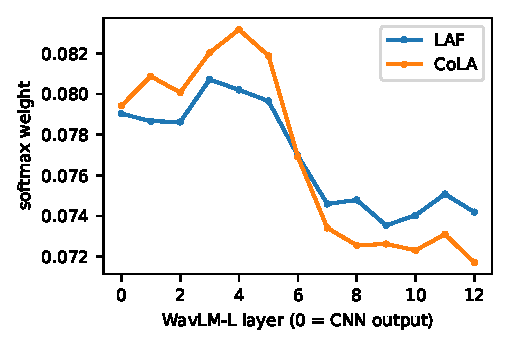
\includegraphics[width=.85\columnwidth]{figs/fig_layers.pdf}}{\fbox{layer weights}}\caption{Learned layer weights (mean over seeds).}\label{fig:layers}\end{figure}
\begin{figure}[t]\centering\IfFileExists{figs/fig_attack_eer.pdf}{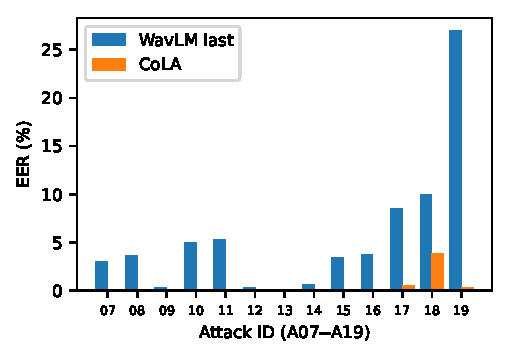
\includegraphics[width=.85\columnwidth]{figs/fig_attack_eer.pdf}}{\fbox{per-attack EER}}\caption{Per-attack EER on LA eval.}\label{fig:attack}\end{figure}
\begin{figure}[t]\centering\IfFileExists{figs/fig_itw_scores.pdf}{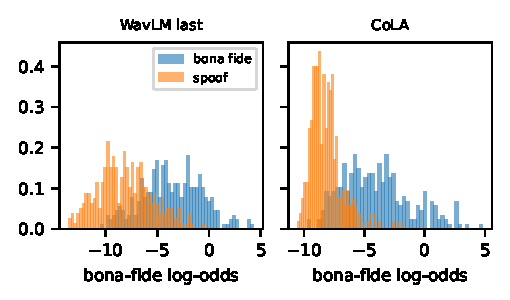
\includegraphics[width=.95\columnwidth]{figs/fig_itw_scores.pdf}}{\fbox{ITW score histograms}}\caption{In-the-Wild score distributions.}\label{fig:hist}\end{figure}

\section{Analysis and Discussion}
\textbf{Explainability.} Fig.~\ref{fig:layers} shows which SSL layers the detector relies on. The learned weights stay close to uniform (0.072--0.083 against $1/13=0.077$), with a slight preference for layers 1--6 over layers 7--12. The gain of LAF therefore appears to come from combining information across all layers rather than from sharp layer selection; the fixed uniform-average control in Table~\ref{tab:main} confirms this. This is consistent with reports that intermediate SSL layers carry useful spoofing cues~\cite{zhang2024sls,pascu2024towards}. \textbf{Error analysis.} Fig.~\ref{fig:attack} gives per-attack EER; For the last-layer baseline the hardest attacks are the voice-conversion attacks A19 (23.7\%), A18 (11.9\%) and A17 (8.4\%). LAF+aug brings all attacks to at most 2.5\% EER; CoLA is similar except A18 (4.4\%) and A15 (1.5\%). Each attack has only about 20 clips in our 600-clip evaluation subset, so per-attack values are noisy. Fig.~\ref{fig:hist} shows the ITW score overlap and calibration shift. \textbf{Why no adversarial gain?} Weights 0.1 and 1.0 were worse than 0.3, so the head is at best neutral and sensitive to its weight. We did not run experiments to identify the cause. Plausible explanations are that the augmentation-type label is only a weak proxy for the real distribution shift between LA and ITW, that $\lambda_{\mathrm{adv}}$ interacts with the small training set (we searched only a coarse grid of three values), or that the fused features already carry little codec information; testing these is left to future work. \textbf{Limitations.} Small CPU-feasible subsets (1000 training clips; 300 dev, 600 LA-eval and 600 ITW clips, class-balanced) and a frozen WavLM-base-plus encoder; seeds share one data subset; no second SSL encoder or re-trained AASIST/SLS baseline; single training corpus; the ITW labels are noisy and clips are cropped to 4\,s; the SSL encoder is frozen; augmentation covers only a few codecs; no ASV-integrated t-DCF on ITW. \textbf{Future work.} Partial fine-tuning/LoRA, vocoder-generated and neural-codec training data~\cite{wang2023vocoded,xu2024codecfake}, ASVspoof~5 evaluation, and calibration.

\section{Conclusion}
We presented a strict LA$\rightarrow$ITW study of all-layer SSL fusion with codec-aware training. All-layer fusion gave the largest improvement (ITW EER 19.7\% to 15.7\%; a fixed uniform average performs comparably), augmentation a smaller one (13.9\%), and the adversarial head none; a gap of about 12 EER points to in-domain performance remains. Code: \url{https://github.com/Shalini-Vasudevan/audio-deepfake-ssl}.

\bibliographystyle{IEEEtran}\bibliography{refs}
\end{document}
